\section{Znaczenie projektu monasca}

\begin{figure}[H]
    \centering
    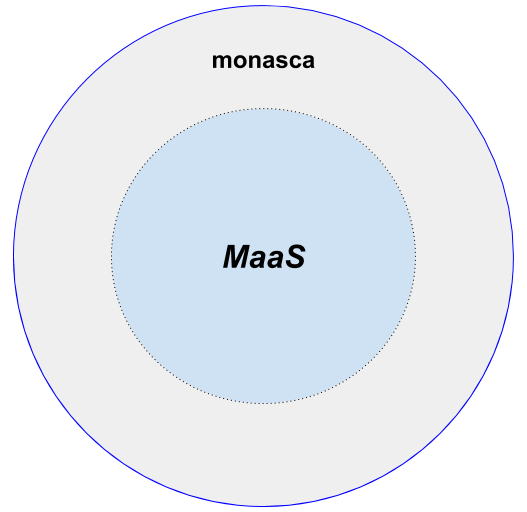
\includegraphics[width=0.6\textwidth]{images/monasca_with_maas}
    \caption[Monasca a paradygmat MaaS]{
        Monasca a paradygmat MaaS, źródło: opracowanie własne
    }
    \label{chapter:application:monasca_and_maas}
\end{figure}

Projekt\textbf{monasca} stanowi praktyczną implementację paradygmatu \textbf{MaaS} 
(rysunek \ref{chapter:application:monasca_and_maas}), składającą się z następujących
programów:
\begin{itemize}
    \item[monasca-api] - REST'owe API, z którym komunikują się pozostałe komponenty, celem zapisywania metryk, alarmów (oraz ich definicji).
    Pozwala także na dostęp do wspomnianych danych.
    \item[monasca-agent] - rozbudowane narzędzie do monitorowania systemu lub aplikacji na maszynie na której został zainstalowany.
    \item[monasca-persister] - prowadzi aktywny nasłuch na kolejce. Wszelkie zmiany stanu na alarmach oraz przekazane metryki, zapisuje,
    poprzez \textbf{monasca-api} do bazy danych.
    \item[monasca-thresh] - jest w stanie, na podstawie zebranych metryk, określić stan w jakim powinien znaleźć się alarm.
    \item[monasca-notification] - na podstawie alarmów, generuje powiadomienie na skonfigurowanego punkty docelowe,
    \item[monasca-ui] - komponent zrealizowany jako wtyczka do \glslink{horizon}{Horizon}, dające wgląd w alarmy, pozwalająca tworzyć ich definicje (monitory).
    Jej główną zaletą jest również wbudowana obsługa do Grafana, która pozwala na przeglądania metryk w czasie rzeczywistym w postaci wykresów.
\end{itemize}

Opisy stos stanowi punkt wyjściowy dla integracji rozwiązania \textbf{LaaS}, głównego
podmiotu poniższej pracy dyplomowej. Ponadto, oprócz wspomnianej rozszerzenia projektu \textbf{monasca}, jest on miejscem kontrybucji programistów Fujitsu, wliczając w to autora
pracy dyplomowej. 